\chapter{Results and Discussion}
The results of our experiments with our data set will be presented in this chapter. 30 runs of each approach that produced feasible solutions are included in the results. Note that some runs produce an infeasible solution. This due to the non-deterministic nature of metaheuristics, which will cause it to produce infeasible solutions sometimes.

\section{Environment}
All of the approaches were run in the following hardware and software configurations:

\begin{itemize}
	\item Hardware
	\begin{itemize}
		\item \textbf{CPU}: Intel Core i3-5010U @ 2.1GHz
		\item \textbf{GPU}: NVIDIA GeForce 920M
		\item \textbf{RAM}: 4GB
	\end{itemize}
	\item Software
	\begin{itemize}
		\item \textbf{OS}: elementaryOS 5.1.7 Hera
		\item \textbf{Linux Kernel Version}: 5.4.0-80-generic
	\end{itemize}
\end{itemize}

\section{Experiments}
We have conducted two sets of experiments in order for us to evaluate the performance of our proposed GWO approach. The first set of experiments varies the GWO parameter, $c$. It shows the impact of the parameter to the algorithm. The second set are experiments with the competing approaches. It shows how our proposed approach compares against other approaches.

\subsection{Results with Different GWO Parameter Values}
Our proposed GWO approach only has one parameter, other than the population size, and number of iterations, the $c$ value. We used four values for the parameter: $2$, $4$, $8$, and $12$. The tables \ref{approach-gwo-c2-results} to \ref{approach-gwo-c12-results} show the results. We will refer to each GWO experiment as $G_{c}$, where $c$ is the value of the $c$ parameter in each experiment. So, the GWO experiment with $c = 2$ will be referred to as $G_{2}$, and so on. Each experiment for each data set has been run 30 times.

\begin{table}[h!]
\begin{adjustwidth}{-1.18in}{}
	\centering
	\begin{tabular}{|l|l|l|l|l|l|}
	\hline
	\multicolumn{1}{|c|}{\multirow{2}{*}{\textbf{Problem}}} & \multicolumn{5}{c|}{\textbf{GWO (c = 2)}} \\ \cline{2-6} 
	\multicolumn{1}{|c|}{}                                  & \multicolumn{1}{c|}{\textbf{Best}} & \multicolumn{1}{c|}{\textbf{Worst}} & \multicolumn{1}{c|}{\textbf{Avg.}} & \multicolumn{1}{c|}{\textbf{Std. Dev.}} & \multicolumn{1}{c|}{\textbf{Avg. Runtime (s)}} \\ \hline
	SFLP-II                                                 & 217.11013                                  & 327.250386                                   & 280.537959566667                      & 25.4125532828332                                 & 89.4666666666667                                  \\ \hline
	mSFLP-III                                               & 50976.368866                                & 60974.152195                                 & 52550.679634						         & 2559.71111762775                              & 252                              \\ \hline
	mKra30a                                               & 90189.743515                               & 115772.751106                                &
	101984.0014387							&
	6124.48412940521							&
	337.666666666667						\\ \hline
	\end{tabular}
\end{adjustwidth}
\caption{Results obtained from our proposed GWO approach with $c = 2$.}
\label{approach-gwo-c2-results}
\end{table}

\begin{table}[h!]
\begin{adjustwidth}{-1.18in}{}
	\centering
	\begin{tabular}{|l|l|l|l|l|l|}
	\hline
	\multicolumn{1}{|c|}{\multirow{2}{*}{\textbf{Problem}}} & \multicolumn{5}{c|}{\textbf{GWO (c = 4)}} \\ \cline{2-6} 
	\multicolumn{1}{|c|}{}                                  & \multicolumn{1}{c|}{\textbf{Best}} & \multicolumn{1}{c|}{\textbf{Worst}} & \multicolumn{1}{c|}{\textbf{Avg.}} & \multicolumn{1}{c|}{\textbf{Std. Dev.}} & \multicolumn{1}{c|}{\textbf{Avg. Runtime (s)}} \\ \hline
	SFLP-II                                                 & 228.686203                                  & 344.260855                                   & 291.886319866667                      & 28.7100369555559                                 & 92.2                                  \\ \hline
	mSFLP-III                                               & 50054.34227                                & 57215.849915                                 & 53477.0850155333						         & 2500.45309541788                              & 223.566666666667                               \\ \hline
	mKra30a                                               & 92722.82975                                & 117413.196259                                 &
	101299.9193804							&
	7045.97218764861							&
	341.733333333333						\\ \hline
	\end{tabular}
\end{adjustwidth}
\caption{Results obtained from our proposed GWO approach with $c = 4$.}
\label{approach-gwo-c4-results}
\end{table}

\begin{table}[h!]
\begin{adjustwidth}{-1.18in}{}
	\centering
	\begin{tabular}{|l|l|l|l|l|l|}
	\hline
	\multicolumn{1}{|c|}{\multirow{2}{*}{\textbf{Problem}}} & \multicolumn{5}{c|}{\textbf{GWO (c = 8)}} \\ \cline{2-6} 
	\multicolumn{1}{|c|}{}                                  & \multicolumn{1}{c|}{\textbf{Best}} & \multicolumn{1}{c|}{\textbf{Worst}} & \multicolumn{1}{c|}{\textbf{Avg.}} & \multicolumn{1}{c|}{\textbf{Std. Dev.}} & \multicolumn{1}{c|}{\textbf{Avg. Runtime (s)}} \\ \hline
	SFLP-II                                                 & 248.460499                                  & 366.977582                                   & 298.4528295                     & 33.2924593371748s                                 & 89.9                                  \\ \hline
	mSFLP-III                                               & 48765.748322                                & 58628.685135                                 & 52961.5490012667						         & 2266.54729594745                              & 221.4                               \\ \hline
	mKra30a                                               & 90284.307087                                & 115441.795624                                 &
	101247.5836841							&
	6943.58470115289							&
	344.066666666667						\\ \hline
	\end{tabular}
\end{adjustwidth}
\caption{Results obtained from our proposed GWO approach with $c = 8$.}
\label{approach-gwo-c8-results}
\end{table}

\begin{table}[h!]
\begin{adjustwidth}{-1.18in}{}
	\centering
	\begin{tabular}{|l|l|l|l|l|l|}
	\hline
	\multicolumn{1}{|c|}{\multirow{2}{*}{\textbf{Problem}}} & \multicolumn{5}{c|}{\textbf{GWO (c = 12)}} \\ \cline{2-6} 
	\multicolumn{1}{|c|}{}                                  & \multicolumn{1}{c|}{\textbf{Best}} & \multicolumn{1}{c|}{\textbf{Worst}} & \multicolumn{1}{c|}{\textbf{Avg.}} & \multicolumn{1}{c|}{\textbf{Std. Dev.}} & \multicolumn{1}{c|}{\textbf{Avg. Runtime (s)}} \\ \hline
	SFLP-II                                                 & 260.756126                                  & 347.908201                                   & 302.537651133333                      & 28.4323476098296                                 & 98.1333333333333                                  \\ \hline
	mSFLP-III                                               & 50026.967411                                & 56354.012672                                 & 51949.7463375						         & 1511.5013830213                              & 228.366666666667                               \\ \hline
	mKra30a                                               & 92347.010582                                & 121198.027782                                 &
	103896.1840302							&
	7555.22717047117							&
	339.566666666667						\\ \hline
	\end{tabular}
\end{adjustwidth}
\caption{Results obtained from our proposed GWO approach with $c = 12$.}
\label{approach-gwo-c12-results}
\end{table}

For SFLP-II, $G_{2}$ has the best average compared to the other experiments, with a value of $280.537959566667$. The other experiments have average of $291.886319866667$, $298.4528295$, and $302.537651133333$ for $G_{4}$, $G_{8}$, and $G_{12}$, respectively. This characteristic is also reflected by the results of the best and worst results of each experiment. $G_{2}$ has the best and worst solutions with fitnesses of $217.11013$ and $327.250386$, respectively. These are better than the other experiments: $228.686203$ and $344.260855$ for $G_{4}$, $248.460499$ and $366.977582$ for $G_{8}$, and $260.756126$ and $347.908201$ for $G_{12}$. The situation is different when we are using mSFLP-III. With $G_{2}$, we have an average fitness of $52550.679634$ and best and worst solutions of $50976.368866$ and $60974.152195$. $G_{4}$ has an average fitness of $53477.0850155333$, with best and worst solutions of $50054.34227$ and $57215.849915$. $G_{8}$ has an average fitness of $52961.5490012667$, with best and worst solutions of $48765.748322$ and $58628.685135$. $G_{12}$ has an average fitness of $51949.7463375$, with best and worst solutions of $50026.967411$ and $56354.012672$. As one can observe, $G_{12}$ provides the best average fitness among the three. Lastly, when using mKra30a, $G_{2}$ provides an average fitness of $101984.0014387$, and best and worst solutions of $90189.743515$ and $115772.751106$. $G_{4}$ provides a better average fitness of $101290.9193804$, and a best and worst solutions of $92722.82975$ and $117413.196259$. $G_{8}$ has an average fitness of $101247.5836841$, and best and worst solutions of $90284.307087$ and $115441.795624$. And finally, $G_{12}$ has an average fitness of $103896.1840302$, and best and worst solutions of $92347.010582$ and $121198.027782$. In this data set, $G_{8}$ provided the best average fitness. Tables \ref{full-data-gwo-c2} to \ref{full-data-gwo-c12} show the entire data we have collected for this set of experiments.

Each data set used in the experiments uses differently-sized bounding regions. For SFLP-II, a $12x12$ bounding region is used. mSFLIP uses a $260x260$ bounding region, while mKra30a uses a $250x250$ one. Notice that $c = 2$ provides the best average fitness for SFLP-II. On the other hand, for mKra30a, $c = 8$ provides the best fitness. Lastly, the best average fitness is given for mSFLP-III when $c = 12$. From this, we can observe that the larger the bounding region, the larger the $c$ parameter values must be in order for us to obtain the best average results as much as possible. As such, we say that the performance of our proposed GWO approach is affected the value of the $c$ parameter, in which the ideal value is dependent on the size of the bounding area. We can attribute this to the fact that the parameter determines how much a building can be shifted away in the formulas of $D_{\alpha}$, $D_{\beta}$, and $D_{\delta}$ (see equations \ref{summary-modified-gwo-a} to \ref{summary-modified-gwo-xt1} in Methodology). A smaller $c$ value introduces a smaller shift, while a larger value will shift the buildings further. In smaller sized bounding regions, a smaller shift is important due to the limited space available. Larger shifts in this size will make it harder for buildings to reach feasibility. On the other hand, a larger shift is more appropriate in a larger space since it will allow buildings to move closer to each other fast. Additionally, such a larger amount of available space can be utilized. A larger space will allow buildings to more easily move away from intersections (and, as a consequence, infeasibility). Later research can focus on determining the ideal $c$ value for a certain bounding region size and identifying whether it can be mathematically modelled instead, rather than being a parameter.

\begin{table}
\centering
\begin{adjustwidth}{}{}
\resizebox{\textwidth}{!}{\rotatebox{90}{
\begin{tabular}{|r|r|r|r|r|r|r|}
\hline
\multicolumn{1}{|c|}{\multirow{2}{*}{Run}} & \multicolumn{6}{c|}{GWO (c = 2)}                                                                                                                                                                                            \\ 
\cline{2-7}
\multicolumn{1}{|c|}{}                     & \multicolumn{1}{l|}{SFLP-II} & \multicolumn{1}{l|}{Elapsed Time (s)} & \multicolumn{1}{l|}{mSFLP-III} & \multicolumn{1}{l|}{Elapsed Time (s)} & \multicolumn{1}{l|}{mKra30a} & \multicolumn{1}{l|}{Elapsed Time (s)}  \\ 
\hline
1                                          & 243.94003                    & 93                                    & 60974.152195                   & 223                                   & 93499.791611                 & 332                                    \\ 
\hline
2                                          & 277.127329                   & 96                                    & 53091.360428                   & 209                                   & 96676.778236                 & 365                                    \\ 
\hline
3                                          & 299.3099                     & 92                                    & 50976.368866                   & 234                                   & 102351.806828                & 341                                    \\ 
\hline
4                                          & 314.957576                   & 93                                    & 51178.316551                   & 208                                   & 110232.681198                & 329                                    \\ 
\hline
5                                          & 280.39426                    & 106                                   & 58477.903175                   & 247                                   & 106633.15947                 & 337                                    \\ 
\hline
6                                          & 275.177478                   & 86                                    & 53929.316643                   & 239                                   & 97451.907082                 & 342                                    \\ 
\hline
7                                          & 277.079203                   & 95                                    & 55831.132965                   & 231                                   & 100241.257439                & 333                                    \\ 
\hline
8                                          & 295.824242                   & 97                                    & 52308.518883                   & 212                                   & 105300.434387                & 331                                    \\ 
\hline
9                                          & 245.953087                   & 90                                    & 53500.27182                    & 219                                   & 105488.929329                & 326                                    \\ 
\hline
10                                         & 293.995934                   & 83                                    & 55547.163464                   & 222                                   & 90189.743515                 & 347                                    \\ 
\hline
11                                         & 327.250386                   & 87                                    & 55864.676971                   & 241                                   & 115772.751106                & 296                                    \\ 
\hline
12                                         & 256.280092                   & 86                                    & 57776.475086                   & 255                                   & 98965.832809                 & 337                                    \\ 
\hline
13                                         & 255.876664                   & 91                                    & 53743.034462                   & 235                                   & 103952.481422                & 347                                    \\ 
\hline
14                                         & 296.138492                   & 98                                    & 51245.876633                   & 240                                   & 93768.24028                  & 319                                    \\ 
\hline
15                                         & 290.668367                   & 97                                    & 51107.24015                    & 232                                   & 101841.903069                & 320                                    \\ 
\hline
16                                         & 303.18901                    & 81                                    & 56488.55666                    & 243                                   & 103972.777603                & 352                                    \\ 
\hline
17                                         & 268.166175                   & 81                                    & 53864.775436                   & 286                                   & 100531.020317                & 336                                    \\ 
\hline
18                                         & 262.328487                   & 94                                    & 52663.234177                   & 228                                   & 97172.480042                 & 308                                    \\ 
\hline
19                                         & 274.764059                   & 80                                    & 58189.777225                   & 224                                   & 105622.637917                & 322                                    \\ 
\hline
20                                         & 265.671289                   & 100                                   & 55662.475075                   & 232                                   & 96604.220119                 & 329                                    \\ 
\hline
21                                         & 245.064429                   & 89                                    & 54614.038124                   & 251                                   & 109968.754013                & 334                                    \\ 
\hline
22                                         & 320.458291                   & 84                                    & 52944.842747                   & 247                                   & 94776.221497                 & 328                                    \\ 
\hline
23                                         & 312.3666                     & 85                                    & 53289.64669                    & 250                                   & 107118.25267                 & 349                                    \\ 
\hline
24                                         & 296.65818                    & 82                                    & 51904.194862                   & 247                                   & 113649.026276                & 342                                    \\ 
\hline
25                                         & 301.040134                   & 88                                    & 51884.295353                   & 223                                   & 96431.615578                 & 347                                    \\ 
\hline
26                                         & 297.75137                    & 84                                    & 53756.719601                   & 225                                   & 99482.437851                 & 339                                    \\ 
\hline
27                                         & 285.689808                   & 87                                    & 56760.790604                   & 245                                   & 101337.518082                & 342                                    \\ 
\hline
28                                         & 217.11013                    & 92                                    & 51268.167229                   & 210                                   & 99809.912193                 & 359                                    \\ 
\hline
29                                         & 269.317118                   & 82                                    & 55126.549274                   & 265                                   & 109009.66539                 & 367                                    \\ 
\hline
30                                         & 266.590667                   & 85                                    & 57035.610909                   & 254                                   & 101665.805832                & 374                                    \\ 
\hline
\multicolumn{1}{|l|}{Average}              & 280.537959566667             & 89.4666666666667                      & 52550.679634                   & 252                                   & 101984.0014387               & 337.666666666667                       \\ 
\hline
\multicolumn{1}{|l|}{Std. Dev}             & 25.4125532828332             & 6.51117518569809                      & 2559.71111762775               & 17.5859465836042                      & 6124.48412940521             & 16.6760892904478                       \\
\hline
\end{tabular}}}
\end{adjustwidth}
\caption{The entire experiment data we have collected using our GWO approach with $c = 2$.}
\label{full-data-gwo-c2}
\end{table}

\begin{table}
\centering
\begin{adjustwidth}{}{}
\resizebox{\textwidth}{!}{\rotatebox{90}{
\begin{tabular}{|r|r|r|r|r|r|r|}
\hline
\multicolumn{1}{|c|}{\multirow{2}{*}{Run}} & \multicolumn{6}{c|}{GWO (c = 4)}                                                                                                                                                                                            \\ 
\cline{2-7}
\multicolumn{1}{|c|}{}                     & \multicolumn{1}{l|}{SFLP-II} & \multicolumn{1}{l|}{Elapsed Time (s)} & \multicolumn{1}{l|}{mSFLP-III} & \multicolumn{1}{l|}{Elapsed Time (s)} & \multicolumn{1}{l|}{mKra30a} & \multicolumn{1}{l|}{Elapsed Time (s)}  \\ 
\hline
1                                          & 325.506968                   & 94                                    & 52732.247017                   & 230                                   & 102461.169735                & 302                                    \\ 
\hline
2                                          & 313.507465                   & 85                                    & 55216.604614                   & 227                                   & 92722.82975                  & 312                                    \\ 
\hline
3                                          & 260.716585                   & 83                                    & 51035.938828                   & 222                                   & 109756.191196                & 329                                    \\ 
\hline
4                                          & 228.686203                   & 85                                    & 51252.923912                   & 235                                   & 94817.31855                  & 319                                    \\ 
\hline
5                                          & 327.630423                   & 84                                    & 50263.415146                   & 231                                   & 98489.470734                 & 357                                    \\ 
\hline
6                                          & 268.685181                   & 91                                    & 51086.920792                   & 234                                   & 94909.669075                 & 320                                    \\ 
\hline
7                                          & 294.791484                   & 93                                    & 52750.471413                   & 224                                   & 95285.917183                 & 313                                    \\ 
\hline
8                                          & 289.043079                   & 86                                    & 55943.949432                   & 201                                   & 95744.025253                 & 345                                    \\ 
\hline
9                                          & 312.831076                   & 110                                   & 52983.088982                   & 216                                   & 96928.298553                 & 344                                    \\ 
\hline
10                                         & 289.53074                    & 109                                   & 57117.076225                   & 219                                   & 104127.696587                & 361                                    \\ 
\hline
11                                         & 306.729307                   & 88                                    & 58398.903725                   & 202                                   & 100803.360954                & 316                                    \\ 
\hline
12                                         & 250.079633                   & 90                                    & 57215.849915                   & 200                                   & 107138.759598                & 334                                    \\ 
\hline
13                                         & 265.35407                    & 91                                    & 52676.416985                   & 224                                   & 99177.543182                 & 360                                    \\ 
\hline
14                                         & 286.189762                   & 102                                   & 54687.376709                   & 218                                   & 116187.673534                & 359                                    \\ 
\hline
15                                         & 344.260855                   & 91                                    & 51621.196281                   & 197                                   & 98794.914215                 & 348                                    \\ 
\hline
16                                         & 312.026299                   & 96                                    & 50204.516571                   & 221                                   & 97385.057663                 & 347                                    \\ 
\hline
17                                         & 308.682295                   & 84                                    & 50423.092026                   & 227                                   & 96082.164837                 & 317                                    \\ 
\hline
18                                         & 276.643616                   & 94                                    & 54081.611893                   & 219                                   & 97633.722404                 & 350                                    \\ 
\hline
19                                         & 313.150303                   & 99                                    & 53775.680328                   & 236                                   & 96896.538696                 & 351                                    \\ 
\hline
20                                         & 269.652821                   & 97                                    & 56298.768982                   & 232                                   & 112493.366562                & 383                                    \\ 
\hline
21                                         & 281.83043                    & 91                                    & 51932.713989                   & 233                                   & 98050.607231                 & 345                                    \\ 
\hline
22                                         & 327.765231                   & 86                                    & 54186.072151                   & 234                                   & 112647.361168                & 367                                    \\ 
\hline
23                                         & 301.150174                   & 96                                    & 56001.447327                   & 228                                   & 106157.126183                & 320                                    \\ 
\hline
24                                         & 236.491096                   & 92                                    & 50493.347454                   & 224                                   & 117413.196259                & 342                                    \\ 
\hline
25                                         & 319.217441                   & 88                                    & 56106.388706                   & 235                                   & 93008.848526                 & 357                                    \\ 
\hline
26                                         & 276.816359                   & 93                                    & 53595.246113                   & 226                                   & 97829.659012                 & 348                                    \\ 
\hline
27                                         & 331.744055                   & 85                                    & 50355.81105                    & 210                                   & 96314.070999                 & 362                                    \\ 
\hline
28                                         & 280.359543                   & 97                                    & 50054.34227                    & 231                                   & 96187.924377                 & 356                                    \\ 
\hline
29                                         & 269.64555                    & 93                                    & 55705.353302                   & 227                                   & 110426.691269                & 357                                    \\ 
\hline
30                                         & 287.871552                   & 93                                    & 56115.778328                   & 244                                   & 103126.408127                & 331                                    \\ 
\hline
\multicolumn{1}{|l|}{Average}              & 291.886319866667             & 92.2                                  & 53477.0850155333               & 223.566666666667                      & 101299.9193804               & 341.733333333333                       \\ 
\hline
\multicolumn{1}{|l|}{Std. Dev}             & 28.7100369555559             & 6.75379842040376                      & 2500.45309541788               & 11.7199603781057                      & 7045.97218764861             & 19.7448087168341                       \\
\hline
\end{tabular}}}
\end{adjustwidth}
\caption{The entire experiment data we have collected using our GWO approach with $c = 4$.}
\label{full-data-gwo-c4}
\end{table}

\begin{table}
\centering
\begin{adjustwidth}{}{}
\resizebox{\textwidth}{!}{\rotatebox{90}{
\begin{tabular}{|r|r|r|r|r|r|r|}
\hline
\multicolumn{1}{|c|}{\multirow{2}{*}{Run}} & \multicolumn{6}{c|}{GWO (c = 8)}                                                                                                                                                                                            \\ 
\cline{2-7}
\multicolumn{1}{|c|}{}                     & \multicolumn{1}{l|}{SFLP-II} & \multicolumn{1}{l|}{Elapsed Time (s)} & \multicolumn{1}{l|}{mSFLP-III} & \multicolumn{1}{l|}{Elapsed Time (s)} & \multicolumn{1}{l|}{mKra30a} & \multicolumn{1}{l|}{Elapsed Time (s)}  \\ 
\hline
1                                          & 248.460499                   & 84                                    & 53610.785446                   & 219                                   & 98898.279633                 & 343                                    \\ 
\hline
2                                          & 274.564365                   & 94                                    & 52513.338478                   & 209                                   & 100419.628815                & 350                                    \\ 
\hline
3                                          & 302.312045                   & 80                                    & 50568.714432                   & 207                                   & 115441.795624                & 383                                    \\ 
\hline
4                                          & 366.977582                   & 82                                    & 50935.866066                   & 196                                   & 101129.673759                & 348                                    \\ 
\hline
5                                          & 351.437374                   & 81                                    & 52687.052628                   & 231                                   & 104964.211197                & 310                                    \\ 
\hline
6                                          & 293.604289                   & 82                                    & 53276.78199                    & 209                                   & 107877.076859                & 330                                    \\ 
\hline
7                                          & 359.01672                    & 80                                    & 48765.748322                   & 208                                   & 94396.735329                 & 338                                    \\ 
\hline
8                                          & 281.076044                   & 80                                    & 54195.000404                   & 218                                   & 101156.75177                 & 325                                    \\ 
\hline
9                                          & 258.799843                   & 83                                    & 51162.727417                   & 210                                   & 100161.090279                & 330                                    \\ 
\hline
10                                         & 309.156362                   & 87                                    & 55257.907051                   & 210                                   & 95184.3936                   & 366                                    \\ 
\hline
11                                         & 298.001013                   & 88                                    & 52524.985062                   & 240                                   & 106860.894058                & 353                                    \\ 
\hline
12                                         & 256.551059                   & 89                                    & 50360.89571                    & 260                                   & 91220.303406                 & 348                                    \\ 
\hline
13                                         & 324.109959                   & 88                                    & 50922.134697                   & 239                                   & 94978.191124                 & 349                                    \\ 
\hline
14                                         & 354.624276                   & 101                                   & 56652.477489                   & 214                                   & 104360.606339                & 376                                    \\ 
\hline
15                                         & 265.625973                   & 87                                    & 53025.049957                   & 227                                   & 93255.101887                 & 325                                    \\ 
\hline
16                                         & 274.332928                   & 85                                    & 54667.90662                    & 236                                   & 109420.16214                 & 338                                    \\ 
\hline
17                                         & 338.788614                   & 83                                    & 54569.908928                   & 229                                   & 100810.654762                & 360                                    \\ 
\hline
18                                         & 316.26818                    & 84                                    & 52833.654724                   & 211                                   & 114560.302063                & 355                                    \\ 
\hline
19                                         & 284.724716                   & 89                                    & 53970.221321                   & 218                                   & 98613.30127                  & 356                                    \\ 
\hline
20                                         & 326.392195                   & 91                                    & 58628.685135                   & 219                                   & 104210.436928                & 321                                    \\ 
\hline
21                                         & 258.933748                   & 96                                    & 55023.283295                   & 223                                   & 96293.000427                 & 317                                    \\ 
\hline
22                                         & 278.549096                   & 95                                    & 51718.918808                   & 221                                   & 95048.400726                 & 349                                    \\ 
\hline
23                                         & 304.88136                    & 101                                   & 53272.755432                   & 223                                   & 95518.153397                 & 340                                    \\ 
\hline
24                                         & 253.959871                   & 94                                    & 50271.951332                   & 210                                   & 101357.740723                & 342                                    \\ 
\hline
25                                         & 266.289299                   & 98                                    & 55870.386436                   & 233                                   & 105547.59832                 & 333                                    \\ 
\hline
26                                         & 305.419387                   & 100                                   & 54329.480991                   & 239                                   & 113965.169518                & 347                                    \\ 
\hline
27                                         & 298.15468                    & 99                                    & 49869.115501                   & 233                                   & 90284.307087                 & 336                                    \\ 
\hline
28                                         & 289.544092                   & 96                                    & 49542.38784                    & 219                                   & 97386.079971                 & 343                                    \\ 
\hline
29                                         & 291.324696                   & 96                                    & 54550.122055                   & 223                                   & 93974.840446                 & 366                                    \\ 
\hline
30                                         & 321.70462                    & 104                                   & 53268.226471                   & 208                                   & 110132.629066                & 345                                    \\ 
\hline
\multicolumn{1}{|l|}{Average}              & 298.4528295                  & 89.9                                  & 52961.5490012667               & 221.4                                 & 101247.5836841               & 344.066666666667                       \\ 
\hline
\multicolumn{1}{|l|}{Std. Dev}             & 33.2924593371748             & 7.38287860876259                      & 2266.54729594745               & 13.4410590715731                      & 6943.58470115289             & 16.6607805698113                       \\
\hline		
\end{tabular}}}
\end{adjustwidth}
\caption{The entire experiment data we have collected using our GWO approach with $c = 8$.}
\label{full-data-gwo-c8}
\end{table}

\begin{table}
\centering
\begin{adjustwidth}{}{}
\resizebox{\textwidth}{!}{\rotatebox{90}{
\begin{tabular}{|r|r|r|r|r|r|r|}
\hline
\multicolumn{1}{|c|}{\multirow{2}{*}{Run}} & \multicolumn{6}{c|}{GWO (c = 12)}                                                                                                                                                                                           \\ 
\cline{2-7}
\multicolumn{1}{|c|}{}                     & \multicolumn{1}{l|}{SFLP-II} & \multicolumn{1}{l|}{Elapsed Time (s)} & \multicolumn{1}{l|}{mSFLP-III} & \multicolumn{1}{l|}{Elapsed Time (s)} & \multicolumn{1}{l|}{mKra30a} & \multicolumn{1}{l|}{Elapsed Time (s)}  \\ 
\hline
1                                          & 325.198625                   & 99                                    & 52047.543182                   & 238                                   & 95841.919846                 & 372                                    \\ 
\hline
2                                          & 324.704731                   & 92                                    & 51689.025543                   & 222                                   & 103786.075714                & 360                                    \\ 
\hline
3                                          & 269.065166                   & 93                                    & 52945.118694                   & 228                                   & 99740.866943                 & 346                                    \\ 
\hline
4                                          & 326.341077                   & 114                                   & 51978.818825                   & 240                                   & 102808.994228                & 359                                    \\ 
\hline
5                                          & 289.15443                    & 95                                    & 52879.366352                   & 204                                   & 97359.653526                 & 358                                    \\ 
\hline
6                                          & 278.748751                   & 87                                    & 51914.836315                   & 222                                   & 111396.818985                & 340                                    \\ 
\hline
7                                          & 260.756126                   & 91                                    & 51006.416012                   & 237                                   & 99269.28125                  & 327                                    \\ 
\hline
8                                          & 284.592043                   & 93                                    & 52387.71917                    & 217                                   & 103900.353561                & 301                                    \\ 
\hline
9                                          & 273.57431                    & 93                                    & 50379.170311                   & 232                                   & 95068.681824                 & 333                                    \\ 
\hline
10                                         & 297.617036                   & 99                                    & 50959.091835                   & 230                                   & 118355.272743                & 353                                    \\ 
\hline
11                                         & 300.946937                   & 100                                   & 56354.012672                   & 236                                   & 94002.354431                 & 350                                    \\ 
\hline
12                                         & 275.701468                   & 90                                    & 51515.804302                   & 211                                   & 92347.010582                 & 347                                    \\ 
\hline
13                                         & 322.800284                   & 83                                    & 53069.496811                   & 207                                   & 94427.751785                 & 354                                    \\ 
\hline
14                                         & 259.122742                   & 87                                    & 51984.823746                   & 200                                   & 102624.565201                & 308                                    \\ 
\hline
15                                         & 347.908201                   & 94                                    & 50026.967411                   & 227                                   & 107260.890884                & 344                                    \\ 
\hline
16                                         & 310.895318                   & 93                                    & 49916.277214                   & 235                                   & 106494.272476                & 353                                    \\ 
\hline
17                                         & 316.526161                   & 117                                   & 50795.31601                    & 230                                   & 118824.088676                & 362                                    \\ 
\hline
18                                         & 296.727487                   & 97                                    & 51147.473198                   & 248                                   & 121198.027782                & 347                                    \\ 
\hline
19                                         & 278.960464                   & 95                                    & 53525.342533                   & 220                                   & 112018.929871                & 341                                    \\ 
\hline
20                                         & 348.199989                   & 97                                    & 50069.230225                   & 250                                   & 102928.725906                & 341                                    \\ 
\hline
21                                         & 291.34798                    & 98                                    & 53924.886276                   & 239                                   & 108919.967438                & 339                                    \\ 
\hline
22                                         & 342.4007                     & 95                                    & 54487.625427                   & 210                                   & 106108.805161                & 338                                    \\ 
\hline
23                                         & 304.986591                   & 100                                   & 50544.047295                   & 238                                   & 99252.132736                 & 366                                    \\ 
\hline
24                                         & 325.226894                   & 116                                   & 50171.551315                   & 225                                   & 109693.997066                & 307                                    \\ 
\hline
25                                         & 319.281647                   & 93                                    & 53062.432899                   & 243                                   & 96151.924267                 & 331                                    \\ 
\hline
26                                         & 266.26707                    & 96                                    & 52427.324341                   & 244                                   & 105429.228325                & 330                                    \\ 
\hline
27                                         & 342.462975                   & 136                                   & 51908.407372                   & 241                                   & 106497.527161                & 320                                    \\ 
\hline
28                                         & 288.818961                   & 98                                    & 49868.087631                   & 236                                   & 101239.117462                & 325                                    \\ 
\hline
29                                         & 262.412588                   & 102                                   & 52228.670654                   & 225                                   & 96223.24498                  & 312                                    \\ 
\hline
30                                         & 345.382782                   & 101                                   & 53277.506554                   & 216                                   & 107715.040096                & 323                                    \\ 
\hline
\multicolumn{1}{|l|}{Average}              & 302.537651133333             & 98.1333333333333                      & 51949.7463375                  & 228.366666666667                      & 103896.1840302               & 339.566666666667                       \\ 
\hline
\multicolumn{1}{|l|}{Std. Dev}             & 28.4323476098296             & 10.5200410820403                      & 1511.5013830213                & 13.2755500784358                      & 7555.22717047117             & 18.369170824553                        \\
\hline
\end{tabular}}}
\end{adjustwidth}
\caption{The entire experiment data we have collected using our GWO approach with $c = 12$.}
\label{full-data-gwo-c12}
\end{table}

\subsection{Results of Other Approaches}
Each approach has their own parameters, and the values we have set for those parameters are shown in Table \ref{approach-parameters}. Both approaches use a population size of 50, and a maximum number of iterations of 400. The following parameter values for the PSO approach were taken from the work of Jolai, F., Tavakkoli-Moghaddam, R., and Taghipour, M. \cite{Jolai2012}.

\begin{table}[h!]
	\centering
	\begin{tabular}{|l|l|l|}
		\hline
		\textbf{Approach}   & \textbf{Parameter} & \textbf{Value} \\ \hline
		GWO                 & c                  & 4              \\ \hline
		\multirow{3}{*}{GA} & Mutation Rate      & 0.05           \\ \cline{2-3} 
		& Tournament Size    & 4              \\ \cline{2-3} 
		& No. of Elites (EN) & 5              \\ \hline
		\multirow{3}{*}{PSO} & w      & 0.05           \\ \cline{2-3} 
		& c1    & 2              \\ \cline{2-3} 
		& c2 	& 2              \\ \hline
	\end{tabular}
	\caption{Parameter values of the GWO, GA, and PSO approaches.}
	\label{approach-parameters}
\end{table}

The results obtained for each approach is shown in Tables \ref{approach-ga-results} to \ref{approach-pso-results}, respectively. As what the tables show, the competing genetic algorithm approach produces a solution that is better than our proposed GWO approach and the PSO approach, with a fitness averages of $274.120352366667$, $50676.8183791$, and $87715.8254635$ for the SFLP-II, mSFLP-III, and mKra30a problem configurations respectively. This is compared to our proposed approach's fitness averages of $291.886319866667$, $53477.0850155333$, and $101299.9193804$. Fortunately for our approach, the PSO approach obtained the fitness averages of $321.292520833333$, $64289.8051163$, and $121057.4221481$, proving that our GWO is not the worst approach. For SFLP-II, the best and worst solutions have fitnesses of $232.839593$ and $353.006875$ for the GA, respectively, compared to our approach's $228.686203$ and $344.260855$. The PSO approach obtained $273.754488$ and $382.774055$. For mSFLP-III, the best and worst solutions have a fitness of $47177.914444$ and $53668.451469$ for the GA, respectively, compared to our approach's $50054.34227$ and $57215.849915$ and the PSO approach's $59673.997963$ and $68433.641548$. Lastly, for mKra30a, the best and worst solutions have fitnesses of $76454.204788$ and $96215.108131$, respectively, for the GA, with our approach obtaining $92722.82975$ and $117413.196259$. PSO produces the poorest best and worst solutions with fitnesses of $107996.773666$ and $131275.843658$. From the results, the competing GA approach is the most stable among the three, basing from the lower standard deviation in all data sets, except for the SFLP-II data set where our approach is the most stable among the three approaches. The GA approach has $31.3302957404409$, $1325.4427345102$, and $4281.86238995314$ for SFLP-II, mSFLP-III, and mKra30a, respectively. This is compared to our approach's $28.710036955555$, $2500.45309541788$, and $7045.97218764861$, and the PSO approach's $32.8103600821748$, $2356.26248290771$, and $5981.21601161922$. This behaviour of producing the best average solution of the GA approach is attributed to the local search methods, which relatively exhaustively finds a better solution in a small area near the best solution found so far in each iteration. These local search methods intensifies the exploitation phase of the approach. Our GWO approach also exploits the local area, but it is not as intensive as the GA approach and only occurs at a later time in a run, similar to how the PSO approach behaves. Notice as well how PSO produces the worst solutions on average among the three. This can be explained with how particles in the PSO approach are equally influenced by their personal best position and their swarm's global best position. This reduces the chances of particles from exploiting the area around the global best position. This behaviour also explains the observation we have with PSO during our experiemnts where the approach struggles to produce good results for the mKra30a data set. It requires multiple runs just to produce a single feasible solution. This is unlike our GWO approach where all wolves are influenced/led by the best three wolves, enabling them to exploit the space around the best found solution. In future studies, different behaviour may be observed when the PSO parameters are tweaked to different values.

\begin{figure}[h!]
\centering
\begin{adjustwidth}{-0.45in}{}
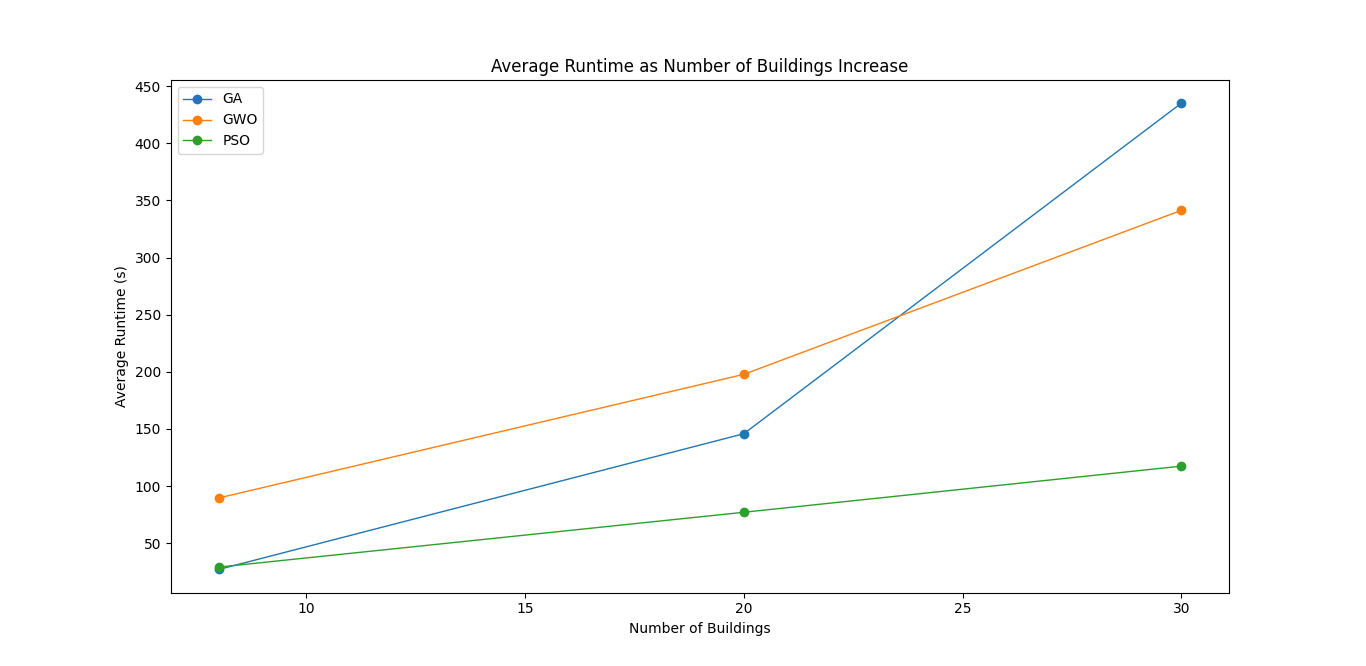
\includegraphics[scale=0.5]{./images/chap07-rd/approaches-average-runtime-over-no-of-buildings.png}
\end{adjustwidth}
\caption{The average runtime (s) of each of the approaches as the number of buildings in a data set increase.}
\label{graph-approaches-runtime-no-buildings}
\end{figure}

The genetic algorithm approach is also the fastest when SFLP-II is being used with an average run time of $27.3666666666667$s, compared to our approach's $92.2$s and the PSO approach's $29.0666666666667$s. However, as the number of buildings increase, the average runtime of the GA approach becomes worse compared to the two other approaches. With mSFLP-III, GA takes $166.866666666667$s, while our approach and the PSO approach takes $223.566666666667$s and $77.0333333333333$s, respectively. GA is still faster than GWO in this data set, but it is already significantly slower than the PSO approach, unlike with the previous data set. Moving towards mKra30a, we can see that GA now takes $455.5$s. This is longer than our approach's $341.733333333333$s, and the PSO approach's $117.4$s. Figure \ref{graph-approaches-runtime-no-buildings} shows this observation. We can attribute this faster increase in average runtime as the number of buildings increase in the GA approach to what enables it produce better solutions on average\textemdash its local search methods. Since the local search methods perform a relatively exhaustive search in order to find a better solution, the GA will take more time to finish executing. Hence, we observe this phenomenon. This is not the case with GWO and PSO, due to the lack of local search methods. GWO may have taken a longer time due to the amount of operations that are performed in the metaheuristic compared to PSO. Better implementations, especially those that utilize SIMD operations, for both approaches may reduce the gap in terms of average run time between the two. However, basing from the equations in both metaheuristics, it is likely that PSO will remain faster than GWO. Further studies, however, are required to exactly determine how well each approach scales with regards to the number of buildings.

\begin{table}[h!]
\begin{adjustwidth}{-1.15in}{}
\centering
\begin{tabular}{|l|l|l|l|l|l|}
	\hline
	\multicolumn{1}{|c|}{\multirow{2}{*}{\textbf{Problem}}} & \multicolumn{5}{c|}{\textbf{Genetic Algorithm}}                                                                                                                                                                                            \\ \cline{2-6} 
	\multicolumn{1}{|c|}{}                                  & \multicolumn{1}{c|}{\textbf{Best}} & \multicolumn{1}{c|}{\textbf{Worst}} & \multicolumn{1}{c|}{\textbf{Avg.}} & \multicolumn{1}{c|}{\textbf{Std. Dev.}} & \multicolumn{1}{c|}{\textbf{Avg. Runtime (s)}} \\ \hline
	SFLP-II                                                 & 232.839593                                  & 353.006875                                   & 274.120352366667                      &
	31.3302957404409						& 27.3666666666667                                   \\ \hline
	mSFLP-III                                               & 47177.914444                               & 53668.451469                                 & 50676.8183791                      & 1325.4427345102                                  & 166.866666666667                           \\ \hline
	mKra30a                                               & 76454.204788                                & 96215.108131                                 &
	87715.8254635							&
	4281.86238995314	                        &
	455.5								\\ \hline
\end{tabular}
\end{adjustwidth}
\caption{Results obtained from using the competing GA approach.}
\label{approach-ga-results}
\end{table}

\begin{table}[h!]
\begin{adjustwidth}{-1.18in}{}
\centering
\begin{tabular}{|l|l|l|l|l|l|}
	\hline
	\multicolumn{1}{|c|}{\multirow{2}{*}{\textbf{Problem}}} & \multicolumn{5}{c|}{\textbf{PSO}} \\ \cline{2-6} 
	\multicolumn{1}{|c|}{}                                  & \multicolumn{1}{c|}{\textbf{Best}} & \multicolumn{1}{c|}{\textbf{Worst}} & \multicolumn{1}{c|}{\textbf{Avg.}} & \multicolumn{1}{c|}{\textbf{Std. Dev.}} & \multicolumn{1}{c|}{\textbf{Avg. Runtime (s)}} \\ \hline
	SFLP-II                                                 & 273.754488                                  & 382.774055                                   &
	321.292520833333							&
	32.8103600821748							&
	29.0666666666667							\\ \hline
	mSFLP-III                                               & 59673.997963                                & 68433.641548                                 &
	64289.8051163					          &
	2356.26248290771						&
	77.0333333333333						\\ \hline
	mKra30a                                               & 107996.773666                                & 131275.843658                                 &
	121057.4221481							&
	5981.21601161922							&
	117.4						\\ \hline
\end{tabular}
\end{adjustwidth}
\caption{Results obtained from our proposed PSO approach.}
\label{approach-pso-results}
\end{table}

We can further obtain insights from our results, by looking at the best solutions generated by each approach. Figures \ref{graph-approaches-best-solutions-sflp-ii} to \ref{graph-approaches-best-solutions-mkra30a} show the fitness graphs of the best solutions using the SFLP-II, mSFLP-III, and mKra30a data sets. The non-linearity of the graph of our GWO approach that is observable in the figures is due to the nature of our approach. All solutions in a population in our approach are replaced after an iteration. Hence, the best solutions may be replaced by poorer solutions. This is unlike with the GA and PSO approaches where  the fitness continuously lower over time. In the case of the GA approach, this is due to the fact that there is elitism. The best $EN$ solutions are kept in the next generation, taking the place of the worst generated solutions produced in the current generation. The PSO approach has a similar characteristic that enables it to produce a continuously lowering fitness graph. In the PSO approach, as discussed before, each particle keeps track of the best position it has found. After an iteration, if a particle finds a position that is better than its personal best, then that position will replace the particle's personal. And if a particle's personal best is better than the swarm's global best, then that position/solution becomes the swarm's global best. It is this global best that is tracked in the graph. The selection procedure of the global best explains the graph of the PSO approach.

\begin{figure}[h!]
\centering
\begin{adjustwidth}{-0.45in}{}
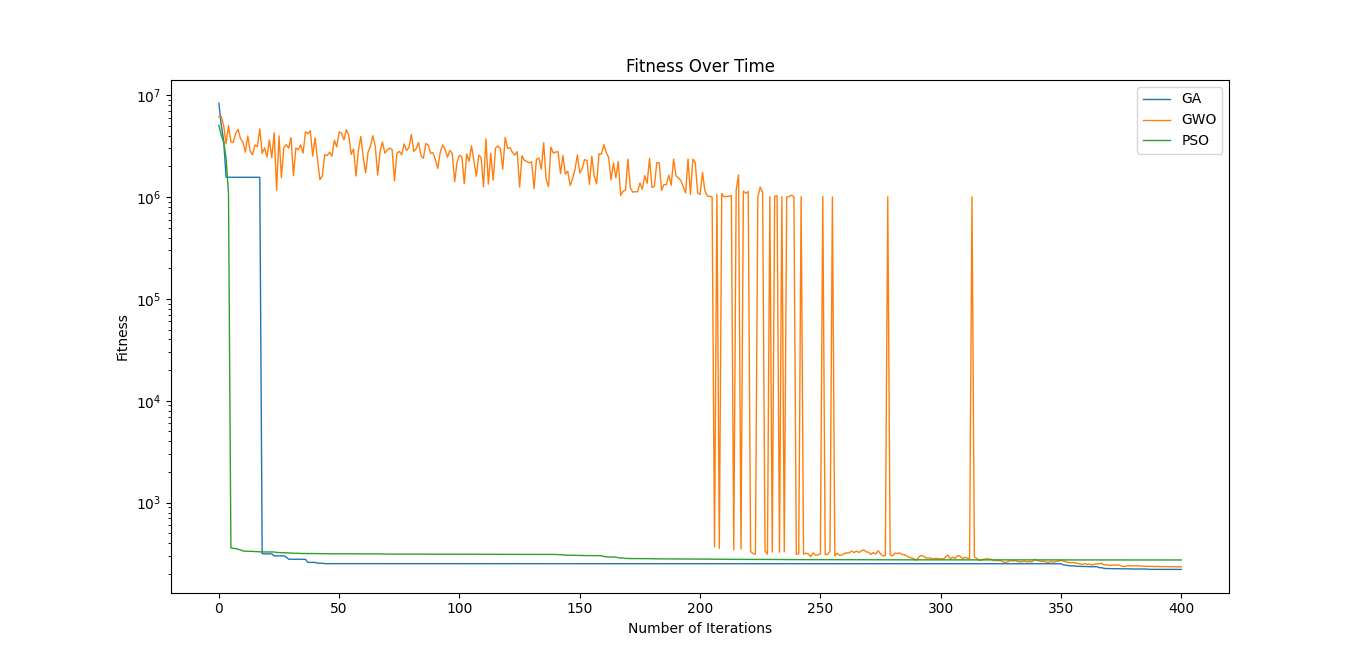
\includegraphics[scale=0.5]{./images/chap07-rd/best-fitness-over-time-sflp2.png}
\end{adjustwidth}
\caption{Fitness over time of the best solutions for the SFLP-II produced by the GA, GWO, and PSO approaches.}
\label{graph-approaches-best-solutions-sflp-ii}
\end{figure}

\begin{figure}[h!]
\centering
\begin{adjustwidth}{-0.45in}{}
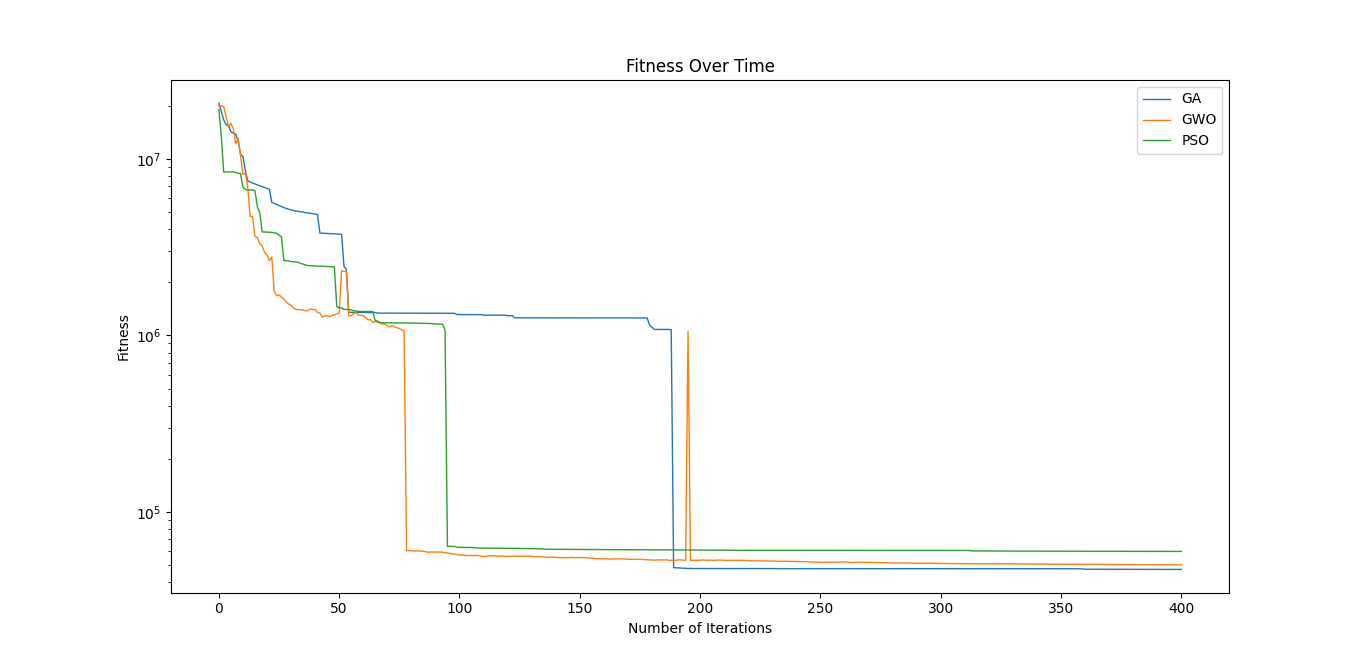
\includegraphics[scale=0.5]{./images/chap07-rd/best-fitness-over-time-msflp3.png}
\end{adjustwidth}
\caption{Fitness over time of the best solutions for the mSFLP-III produced by the GA, GWO, and PSO approaches.}
\label{graph-approaches-best-solutions-msflp-iii}
\end{figure}

\begin{figure}[h!]
\centering
\begin{adjustwidth}{-0.45in}{}
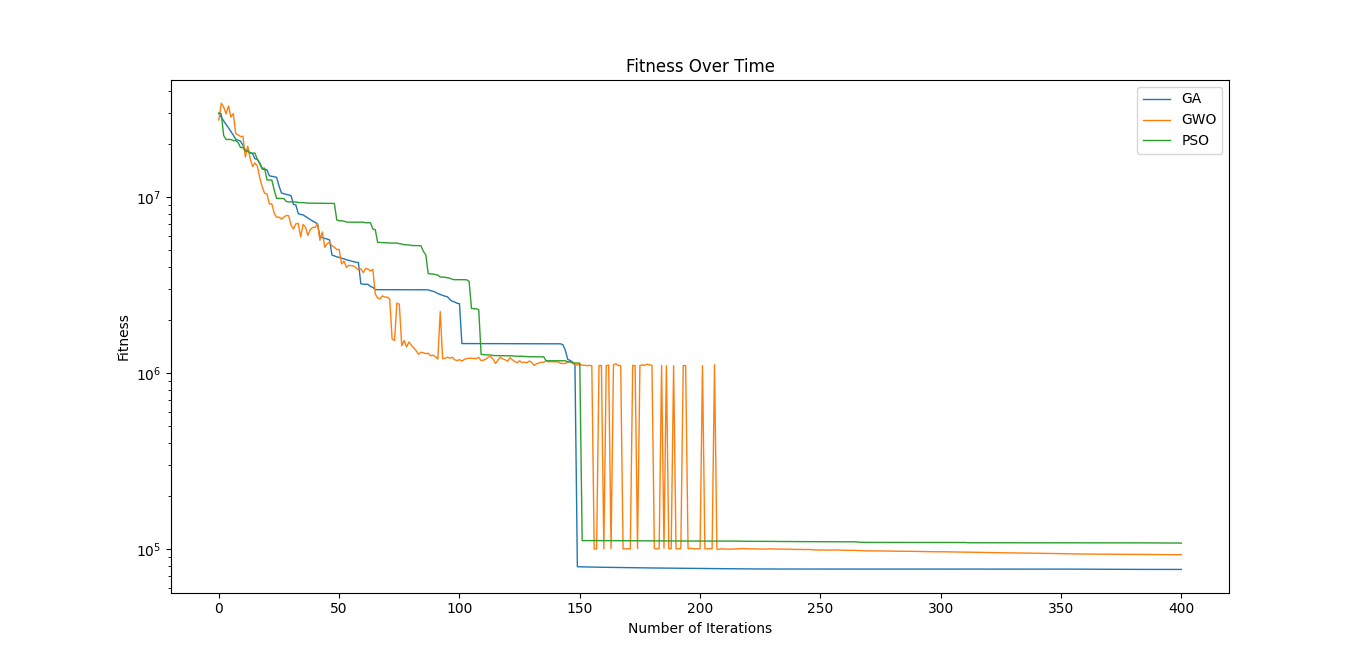
\includegraphics[scale=0.5]{./images/chap07-rd/best-fitness-over-time-mKra30a.png}
\end{adjustwidth}
\caption{Fitness over time of the best solutions for the mKra30a produced by the GA, GWO, and PSO approaches.}
\label{graph-approaches-best-solutions-mkra30a}
\end{figure}

Another avenue we can use to gather insights is through the visualization of the results produced by the approaches mentioned in this study. Figures \ref{best-results-ga} to \ref{best-results-pso} show a visualization of the best results. Notice that with the hybrid GA approach and our GWO approach, the buildings tend to clump together, which is what we want to happen, based on our objective function. For our hybrid GA approach, we can attribute the result to the local search method as well as the mutation operators as they were key to ensure that the buildings are close to each other. The crossover operator is also instrumental in achieving this result by finding combinations that will lead to the result. Our GWO approach also makes buildings clump together but not to the same degree as the GA approach, as can be observed from one building being far from the rest of the buildings in mKra30a data set in Figure \ref{best-results-gwo}. The clumping ability of our approach is attributable to how solutions are allowed to perturb their buildings to positions relatively far from the buildings positions in the best three solution initially. Eventually, our approach will decrease the distance of the buildings in a solution from the leading solutions. Remember that the leading solutions eventually become similar to each other, which help drive the reduction of the degree of building shifting. This gradually decreasing shifting of the buildings will lead to intersections from being resolved and reducing the distance of buildings from each other. The intersections are resolved by reducing the chances of buildings being to moved to a relatively further position where they would still intersect with another building, and gradually pushing intersecting buildings away from each other towards non-intersection. Note that the objective function has a lower penalty for solutions with buildings that do not significantly intersect. The decreasing shifting also encourages buildings to move towards each other due to the fact that smaller shifts have lower probability of causing buildings to intersect with one another too deeply or at all, which allows buildings to move to positions that are closer to the other buildings but without any intersections. Finally, as one can notice in Figure \ref{best-results-pso}, the PSO approach struggles to produce a solution where the buildings are clumped together. This deficiency is not necessarily clear with a small number of buildings, but it does as the number increases. We can attribute this difficulty of the PSO approach to the fact that the buildings are continuously being influenced on the same degree throughout all of the iterations by a particle's personal best and the swarm's global best. This encourages more exploitation and fewer exploitation. As a result, this reduces the chances in which buildings would be able to shift their positions by a small amount, making it more difficult for the approach to find better solutions and have buildings clump together.

\begin{figure}[h!]
\centering
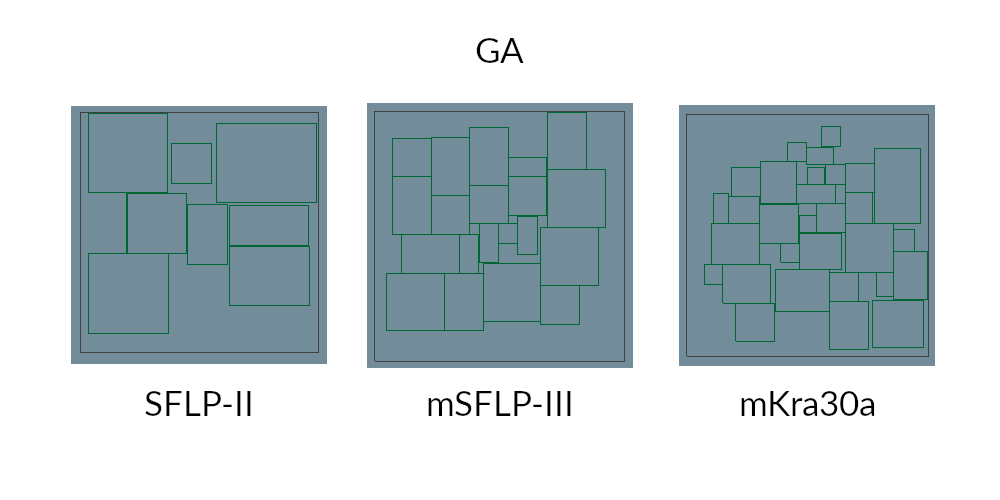
\includegraphics[scale=1.85]{./images/chap07-rd/ga-best-solutions.png}
\caption{Visualization of the best solutions produced by the hybrid GA approach for the three data sets used in this study.}
\label{best-results-ga}
\end{figure}

\begin{figure}[h!]
\centering
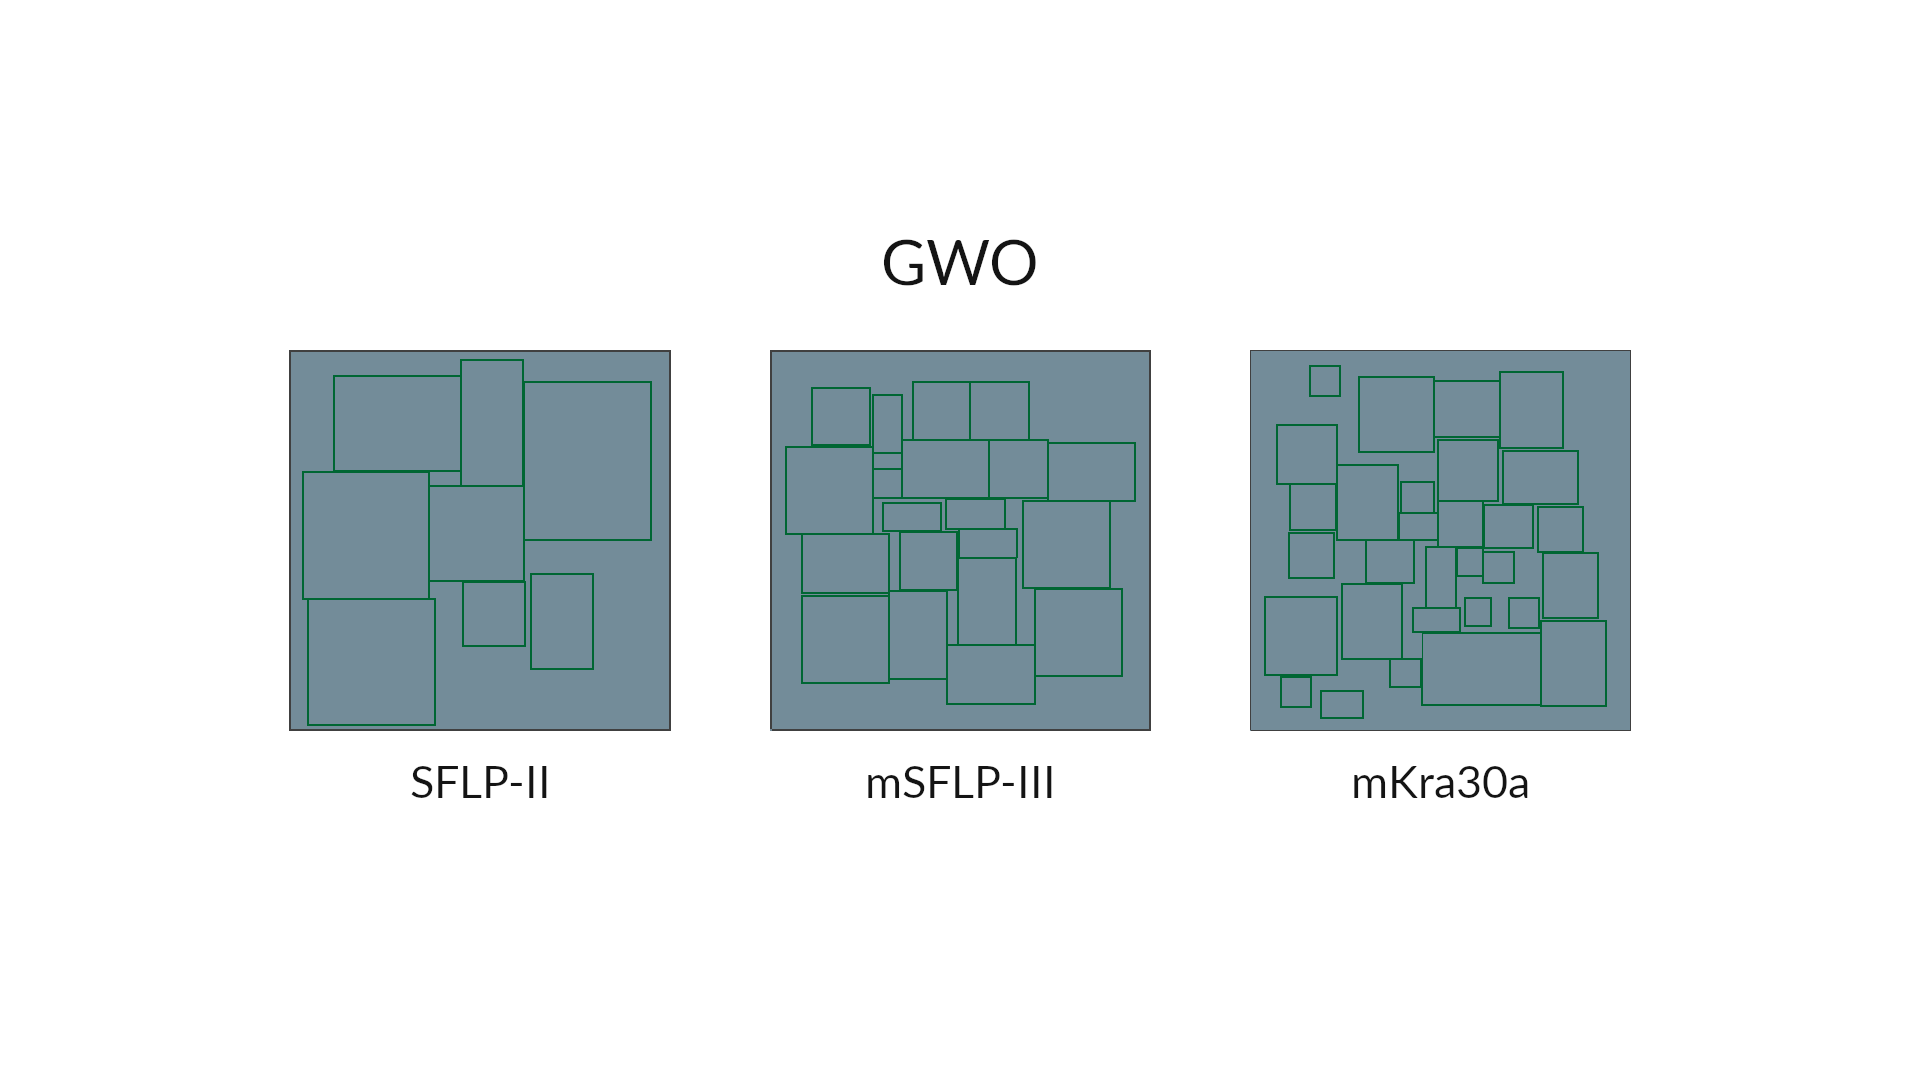
\includegraphics[scale=1.85]{./images/chap07-rd/gwo-best-solutions.png}
\caption{Visualization of the best solutions produced by our GWO approach for the three data sets used in this study.}
\label{best-results-gwo}
\end{figure}

\begin{figure}[h!]
\centering
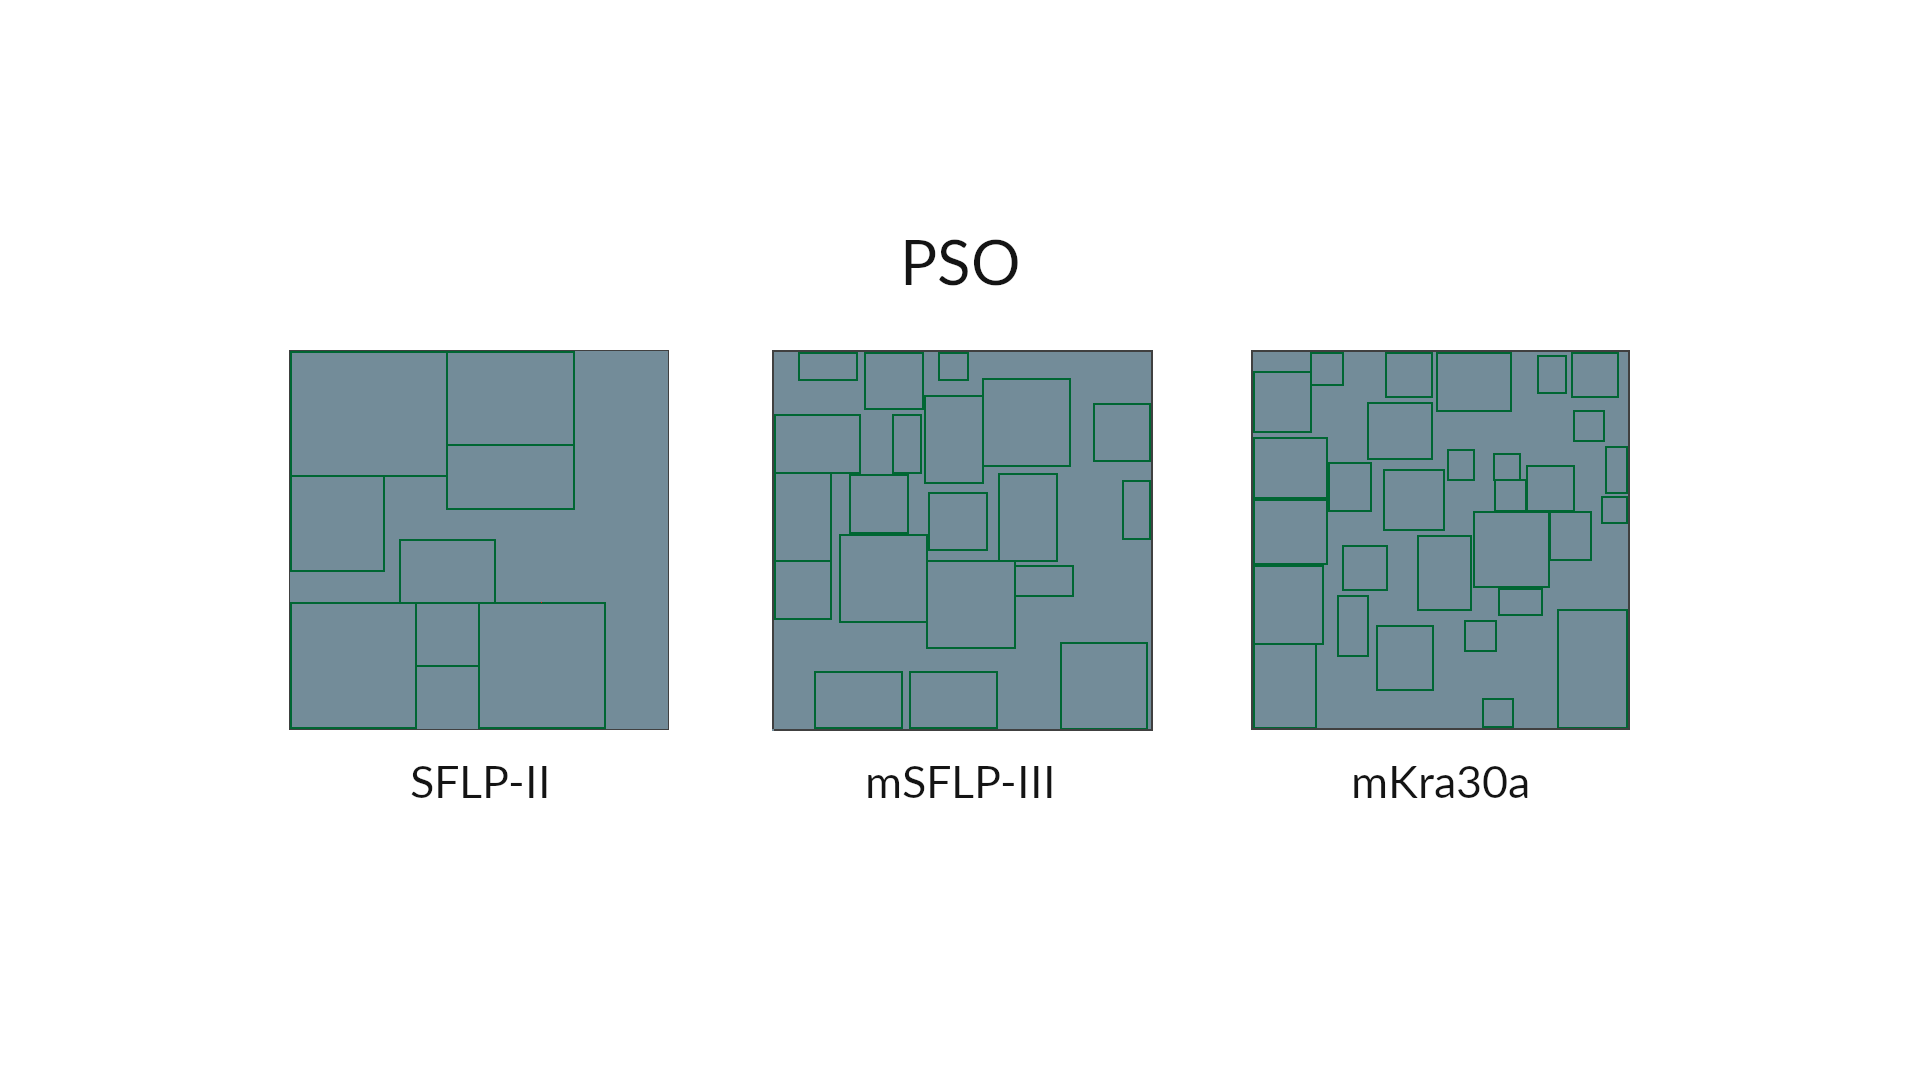
\includegraphics[scale=1.85]{./images/chap07-rd/pso-best-solutions.png}
\caption{Visualization of the best solutions produced by the PSO approach for the three data sets used in this study.}
\label{best-results-pso}
\end{figure}

For reference, tables \ref{full-data-ga} to \ref{full-data-pso} provide the detailed numbers we have obtained in our experiments for each approach and data set. Table \ref{full-data-ga} shows the entire experiment data for our hybrid GA approach, table \ref{full-data-gwo} shows the data for our GWO approach, and lastly, table \ref{full-data-pso} shows the data for the PSO approach.

\begin{table}
\centering
\begin{adjustwidth}{}{}
\resizebox{\textwidth}{!}{\rotatebox{90}{
\begin{tabular}{|r|r|r|r|r|r|r|} 
\hline
\multicolumn{1}{|c|}{\multirow{2}{*}{Run}} & \multicolumn{6}{c|}{GA Experimental Results}                                                                                                                                                                          \\ 
\cline{2-7}
\multicolumn{1}{|c|}{}                     & \multicolumn{1}{l|}{SFLP-II} & \multicolumn{1}{l|}{Elapsed Time (s)} & \multicolumn{1}{l|}{mSFLP-III} & \multicolumn{1}{l|}{Elapsed Time (s)} & \multicolumn{1}{l|}{mKra30a} & \multicolumn{1}{l|}{Elapsed Time (s)}  \\ 
\hline
1                                          & 241.353251                   & 31                                    & 51469.406654                   & 155                                   & 76454.204788                 & 417                                    \\ 
\hline
2                                          & 260.666385                   & 27                                    & 50203.262684                   & 166                                   & 90215.278652                 & 454                                    \\ 
\hline
3                                          & 317.934947                   & 34                                    & 49903.403969                   & 159                                   & 80078.077255                 & 442                                    \\ 
\hline
4                                          & 257.12075                    & 26                                    & 51214.094765                   & 149                                   & 85424.753021                 & 453                                    \\ 
\hline
5                                          & 252.747648                   & 26                                    & 49754.550606                   & 152                                   & 85276.805458                 & 416                                    \\ 
\hline
6                                          & 291.574655                   & 27                                    & 49526.201752                   & 160                                   & 88156.523018                 & 472                                    \\ 
\hline
7                                          & 292.021864                   & 27                                    & 49669.613991                   & 157                                   & 83149.07745                  & 423                                    \\ 
\hline
8                                          & 281.474234                   & 27                                    & 51731.675354                   & 176                                   & 88411.142647                 & 413                                    \\ 
\hline
9                                          & 269.290927                   & 26                                    & 51245.732857                   & 172                                   & 90734.373741                 & 478                                    \\ 
\hline
10                                         & 269.423721                   & 27                                    & 48920.435341                   & 175                                   & 87220.602196                 & 488                                    \\ 
\hline
11                                         & 240.832309                   & 26                                    & 52856.025909                   & 212                                   & 81419.135918                 & 446                                    \\ 
\hline
12                                         & 259.251911                   & 24                                    & 49490.654926                   & 144                                   & 89084.201248                 & 498                                    \\ 
\hline
13                                         & 257.123175                   & 27                                    & 51225.387764                   & 164                                   & 82219.564217                 & 449                                    \\ 
\hline
14                                         & 232.839593                   & 26                                    & 49141.684452                   & 197                                   & 91560.704735                 & 440                                    \\ 
\hline
15                                         & 305.979567                   & 27                                    & 52062.448891                   & 161                                   & 85431.277306                 & 446                                    \\ 
\hline
16                                         & 263.951872                   & 26                                    & 51269.011093                   & 175                                   & 93689.351776                 & 451                                    \\ 
\hline
17                                         & 271.432117                   & 25                                    & 52881.041428                   & 176                                   & 85395.590744                 & 431                                    \\ 
\hline
18                                         & 278.044098                   & 33                                    & 51087.689514                   & 180                                   & 87894.849144                 & 421                                    \\ 
\hline
19                                         & 266.951438                   & 28                                    & 51001.627296                   & 171                                   & 91152.267059                 & 445                                    \\ 
\hline
20                                         & 246.816533                   & 27                                    & 50198.549866                   & 178                                   & 88895.677979                 & 471                                    \\ 
\hline
21                                         & 275.481676                   & 27                                    & 50003.058311                   & 162                                   & 87140.735931                 & 468                                    \\ 
\hline
22                                         & 353.006875                   & 26                                    & 51480.186226                   & 162                                   & 88911.361496                 & 533                                    \\ 
\hline
23                                         & 336.045243                   & 26                                    & 51068.014679                   & 182                                   & 88503.003464                 & 499                                    \\ 
\hline
24                                         & 267.427919                   & 28                                    & 53668.451469                   & 177                                   & 90751.106781                 & 487                                    \\ 
\hline
25                                         & 318.71513                    & 28                                    & 49688.022858                   & 167                                   & 87554.161316                 & 480                                    \\ 
\hline
26                                         & 239.385818                   & 31                                    & 50890.728996                   & 161                                   & 89753.353699                 & 516                                    \\ 
\hline
27                                         & 235.181557                   & 27                                    & 51466.78817                    & 160                                   & 92770.250797                 & 431                                    \\ 
\hline
28                                         & 256.815948                   & 27                                    & 47177.914444                   & 159                                   & 93206.425659                 & 443                                    \\ 
\hline
29                                         & 329.646141                   & 27                                    & 50171.089684                   & 146                                   & 84805.798279                 & 473                                    \\ 
\hline
30                                         & 255.073269                   & 27                                    & 49837.797424                   & 151                                   & 96215.108131                 & 381                                    \\ 
\hline
\multicolumn{1}{|l|}{Average}              & 274.120352366667             & 27.3666666666667                      & 50676.8183791                  & 166.866666666667                      & 87715.8254635                & 455.5                                  \\ 
\hline
\multicolumn{1}{|l|}{Std. Dev}             & 31.3302957404409             & 2.17324377503931                      & 1325.4427345102                & 14.6775299372024                      & 4281.86238995314             & 33.3639801644497                       \\
\hline
\end{tabular}}}
\end{adjustwidth}
\caption{The entire experiment data we have collected using our hybrid GA approach.}
\label{full-data-ga}
\end{table}

\begin{table}
\centering
\begin{adjustwidth}{}{}
\resizebox{\textwidth}{!}{\rotatebox{90}{
\begin{tabular}{|r|r|r|r|r|r|r|} 
\hline
\multicolumn{1}{|c|}{\multirow{2}{*}{Run}} & \multicolumn{6}{c|}{GWO Experimental Results}                                                                                                                                                                         \\ 
\cline{2-7}
\multicolumn{1}{|c|}{}                     & \multicolumn{1}{l|}{SFLP-II} & \multicolumn{1}{l|}{Elapsed Time (s)} & \multicolumn{1}{l|}{mSFLP-III} & \multicolumn{1}{l|}{Elapsed Time (s)} & \multicolumn{1}{l|}{mKra30a} & \multicolumn{1}{l|}{Elapsed Time (s)}  \\ 
\hline
1                                          & 325.506968                   & 94                                    & 52732.247017                   & 230                                   & 102461.169735                & 302                                    \\ 
\hline
2                                          & 313.507465                   & 85                                    & 55216.604614                   & 227                                   & 92722.82975                  & 312                                    \\ 
\hline
3                                          & 260.716585                   & 83                                    & 51035.938828                   & 222                                   & 109756.191196                & 329                                    \\ 
\hline
4                                          & 228.686203                   & 85                                    & 51252.923912                   & 235                                   & 94817.31855                  & 319                                    \\ 
\hline
5                                          & 327.630423                   & 84                                    & 50263.415146                   & 231                                   & 98489.470734                 & 357                                    \\ 
\hline
6                                          & 268.685181                   & 91                                    & 51086.920792                   & 234                                   & 94909.669075                 & 320                                    \\ 
\hline
7                                          & 294.791484                   & 93                                    & 52750.471413                   & 224                                   & 95285.917183                 & 313                                    \\ 
\hline
8                                          & 289.043079                   & 86                                    & 55943.949432                   & 201                                   & 95744.025253                 & 345                                    \\ 
\hline
9                                          & 312.831076                   & 110                                   & 52983.088982                   & 216                                   & 96928.298553                 & 344                                    \\ 
\hline
10                                         & 289.53074                    & 109                                   & 57117.076225                   & 219                                   & 104127.696587                & 361                                    \\ 
\hline
11                                         & 306.729307                   & 88                                    & 58398.903725                   & 202                                   & 100803.360954                & 316                                    \\ 
\hline
12                                         & 250.079633                   & 90                                    & 57215.849915                   & 200                                   & 107138.759598                & 334                                    \\ 
\hline
13                                         & 265.35407                    & 91                                    & 52676.416985                   & 224                                   & 99177.543182                 & 360                                    \\ 
\hline
14                                         & 286.189762                   & 102                                   & 54687.376709                   & 218                                   & 116187.673534                & 359                                    \\ 
\hline
15                                         & 344.260855                   & 91                                    & 51621.196281                   & 197                                   & 98794.914215                 & 348                                    \\ 
\hline
16                                         & 312.026299                   & 96                                    & 50204.516571                   & 221                                   & 97385.057663                 & 347                                    \\ 
\hline
17                                         & 308.682295                   & 84                                    & 50423.092026                   & 227                                   & 96082.164837                 & 317                                    \\ 
\hline
18                                         & 276.643616                   & 94                                    & 54081.611893                   & 219                                   & 97633.722404                 & 350                                    \\ 
\hline
19                                         & 313.150303                   & 99                                    & 53775.680328                   & 236                                   & 96896.538696                 & 351                                    \\ 
\hline
20                                         & 269.652821                   & 97                                    & 56298.768982                   & 232                                   & 112493.366562                & 383                                    \\ 
\hline
21                                         & 281.83043                    & 91                                    & 51932.713989                   & 233                                   & 98050.607231                 & 345                                    \\ 
\hline
22                                         & 327.765231                   & 86                                    & 54186.072151                   & 234                                   & 112647.361168                & 367                                    \\ 
\hline
23                                         & 301.150174                   & 96                                    & 56001.447327                   & 228                                   & 106157.126183                & 320                                    \\ 
\hline
24                                         & 236.491096                   & 92                                    & 50493.347454                   & 224                                   & 117413.196259                & 342                                    \\ 
\hline
25                                         & 319.217441                   & 88                                    & 56106.388706                   & 235                                   & 93008.848526                 & 357                                    \\ 
\hline
26                                         & 276.816359                   & 93                                    & 53595.246113                   & 226                                   & 97829.659012                 & 348                                    \\ 
\hline
27                                         & 331.744055                   & 85                                    & 50355.81105                    & 210                                   & 96314.070999                 & 362                                    \\ 
\hline
28                                         & 280.359543                   & 97                                    & 50054.34227                    & 231                                   & 96187.924377                 & 356                                    \\ 
\hline
29                                         & 269.64555                    & 93                                    & 55705.353302                   & 227                                   & 110426.691269                & 357                                    \\ 
\hline
30                                         & 287.871552                   & 93                                    & 56115.778328                   & 244                                   & 103126.408127                & 331                                    \\ 
\hline
\multicolumn{1}{|l|}{Average}              & 291.886319866667             & 92.2                                  & 53477.0850155333               & 223.566666666667                      & 101299.9193804               & 341.733333333333                       \\ 
\hline
\multicolumn{1}{|l|}{Std. Dev}             & 28.7100369555559             & 6.75379842040376                      & 2500.45309541788               & 11.7199603781057                      & 7045.97218764861             & 19.7448087168341                       \\
\hline
\end{tabular}}}
\end{adjustwidth}
\caption{The entire experiment data we have collected using our hybrid GWO approach.}
\label{full-data-gwo}
\end{table}

\begin{table}
\centering
\begin{adjustwidth}{}{}
\resizebox{\textwidth}{!}{\rotatebox{90}{
\begin{tabular}{|r|r|r|r|r|r|r|} 
\hline
\multicolumn{1}{|c|}{\multirow{2}{*}{Run}} & \multicolumn{6}{c|}{PSO Experimental Results}                                                                                                                                                                         \\ 
\cline{2-7}
\multicolumn{1}{|c|}{}                     & \multicolumn{1}{l|}{SFLP-II} & \multicolumn{1}{l|}{Elapsed Time (s)} & \multicolumn{1}{l|}{mSFLP-III} & \multicolumn{1}{l|}{Elapsed Time (s)} & \multicolumn{1}{l|}{mKra30a} & \multicolumn{1}{l|}{Elapsed Time (s)}  \\ 
\hline
1                                          & 318.852793                   & 30                                    & 64984.15004                    & 76                                    & 126400.957298                & 130                                    \\ 
\hline
2                                          & 322.977083                   & 28                                    & 65613.267347                   & 81                                    & 121843.241837                & 115                                    \\ 
\hline
3                                          & 319.688772                   & 27                                    & 66182.148331                   & 77                                    & 131064.62114                 & 117                                    \\ 
\hline
4                                          & 382.774055                   & 29                                    & 65321.947243                   & 74                                    & 123193.080185                & 109                                    \\ 
\hline
5                                          & 328.181972                   & 26                                    & 68316.333054                   & 90                                    & 113509.606079                & 116                                    \\ 
\hline
6                                          & 273.754488                   & 27                                    & 63051.351074                   & 80                                    & 126382.984985                & 104                                    \\ 
\hline
7                                          & 277.929458                   & 35                                    & 64844.383484                   & 80                                    & 118793.658676                & 113                                    \\ 
\hline
8                                          & 333.791855                   & 29                                    & 62119.790359                   & 78                                    & 116690.745407                & 115                                    \\ 
\hline
9                                          & 331.588456                   & 25                                    & 62520.697372                   & 81                                    & 112328.409836                & 114                                    \\ 
\hline
10                                         & 312.062043                   & 28                                    & 60370.992424                   & 70                                    & 125547.949913                & 117                                    \\ 
\hline
11                                         & 347.300041                   & 26                                    & 63191.887421                   & 74                                    & 128467.742325                & 111                                    \\ 
\hline
12                                         & 276.72711                    & 29                                    & 66079.518539                   & 75                                    & 115259.262817                & 123                                    \\ 
\hline
13                                         & 346.501261                   & 38                                    & 68433.641548                   & 72                                    & 120682.394836                & 123                                    \\ 
\hline
14                                         & 324.057936                   & 29                                    & 59673.997963                   & 73                                    & 115606.839714                & 136                                    \\ 
\hline
15                                         & 294.477526                   & 33                                    & 65232.604935                   & 77                                    & 107996.773666                & 135                                    \\ 
\hline
16                                         & 354.944439                   & 28                                    & 62623.302681                   & 77                                    & 117466.287628                & 119                                    \\ 
\hline
17                                         & 278.580433                   & 25                                    & 63571.512451                   & 78                                    & 119787.763885                & 111                                    \\ 
\hline
18                                         & 373.62812                    & 25                                    & 65604.954414                   & 73                                    & 121933.62674                 & 111                                    \\ 
\hline
19                                         & 277.326199                   & 27                                    & 60121.135582                   & 71                                    & 120619.96003                 & 128                                    \\ 
\hline
20                                         & 312.888415                   & 26                                    & 65799.8442                     & 77                                    & 114528.809418                & 112                                    \\ 
\hline
21                                         & 349.500618                   & 28                                    & 62835.800159                   & 86                                    & 123371.321442                & 113                                    \\ 
\hline
22                                         & 324.432381                   & 30                                    & 67968.856182                   & 80                                    & 125755.185791                & 107                                    \\ 
\hline
23                                         & 259.640869                   & 29                                    & 61263.364929                   & 77                                    & 114837.336021                & 109                                    \\ 
\hline
24                                         & 324.809072                   & 28                                    & 64277.566399                   & 78                                    & 119911.446892                & 114                                    \\ 
\hline
25                                         & 315.892269                   & 30                                    & 63997.453415                   & 72                                    & 130395.024284                & 101                                    \\ 
\hline
26                                         & 367.985685                   & 31                                    & 62791.55909                    & 73                                    & 126777.9534                  & 109                                    \\ 
\hline
27                                         & 306.720735                   & 37                                    & 66069.317642                   & 77                                    & 116590.569717                & 132                                    \\ 
\hline
28                                         & 373.704857                   & 29                                    & 65694.84201                    & 77                                    & 131275.843658                & 145                                    \\ 
\hline
29                                         & 288.776388                   & 30                                    & 67406.459572                   & 76                                    & 118132.533211                & 120                                    \\ 
\hline
30                                         & 339.280296                   & 30                                    & 62731.473629                   & 81                                    & 126570.733612                & 113                                    \\ 
\hline
\multicolumn{1}{|l|}{Average}              & 321.292520833333             & 29.0666666666667                      & 64289.8051163                  & 77.0333333333333                      & 121057.4221481               & 117.4                                  \\ 
\hline
\multicolumn{1}{|l|}{Std. Dev}             & 32.8103600821748             & 3.20488133443597                      & 2356.26248290771               & 4.29501180868943                      & 5981.21601161922             & 10.1526283330459                       \\
\hline
\end{tabular}}}
\end{adjustwidth}
\caption{The entire experiment data we have collected using our hybrid PSO approach.}
\label{full-data-pso}
\end{table}

The performance of the GA approach in this study is definitely noteworthy. It produces the best solutions on average among the three approaches. However, based on the results, the GA approach does not scale well as the number of buildings increase, compared to our approach and the PSO approach. PSO definitely shows the best average runtimes. However, it produces the worst average fitness. For faster speed, we traded performance. This is where our approach shines. Our approach is the second best when it comes to solution quality as the problem scales higher. It is also the second best in terms of speed. This shows to us that our GWO approach provides a balance between speed and performance. Our approach also requires only a few parameters. We argue that this will simplify and speed up experimental setups and configuration in later studies and applications. Importantly, the results also indicate that there is promise in further exploring the applicability of the grey wolf optimization algorithm in solving the facility layout problem.

